\documentclass[conference]{IEEEtran}
%\renewcommand{\thesubsection}{\thesection.\alph{subsection}}

%\addtolength{\oddsidemargin}{-.875in}
%\addtolength{\evensidemargin}{-.875in}
%\addtolength{\textwidth}{1.75in}
%\addtolength{\topmargin}{-.875in}
%\addtolength{\textheight}{1.75in}
	
\usepackage{bm}
\usepackage{amsmath}
\usepackage{amssymb}
\usepackage{tikz}
\usetikzlibrary{automata,positioning}
\usepackage{url}
\usepackage{float}
\usepackage{setspace}
\usepackage{filecontents,lipsum}
\usepackage[noadjust]{cite}
\usepackage{listings}

\begin{document}
%\raggedright
%\doublespacing

\title{A Survey on Machine Learning and Antipatterns}
\author{Rodger Byrd}
\maketitle

\section{Abstract}
\section{Background}
\subsection{Code Smells vs Anti Patterns}
\subsection{Machine Learning}

\subsection{Journal3}
\subsection{Topic Map}
For my area I'm looking at Anti-Patterns in code, these are also known as code smells. I've also seen them referred to as Atoms of Confusion and nano patterrns. My topic map is included below in figure \ref{fig:TM}. My thoughts on gaps are some method to demonstrate the found anti-patterns are valid. Also, there seems to be a gap in how to fix anti-patterns and code smells. 
\begin{figure*}
  \centerline{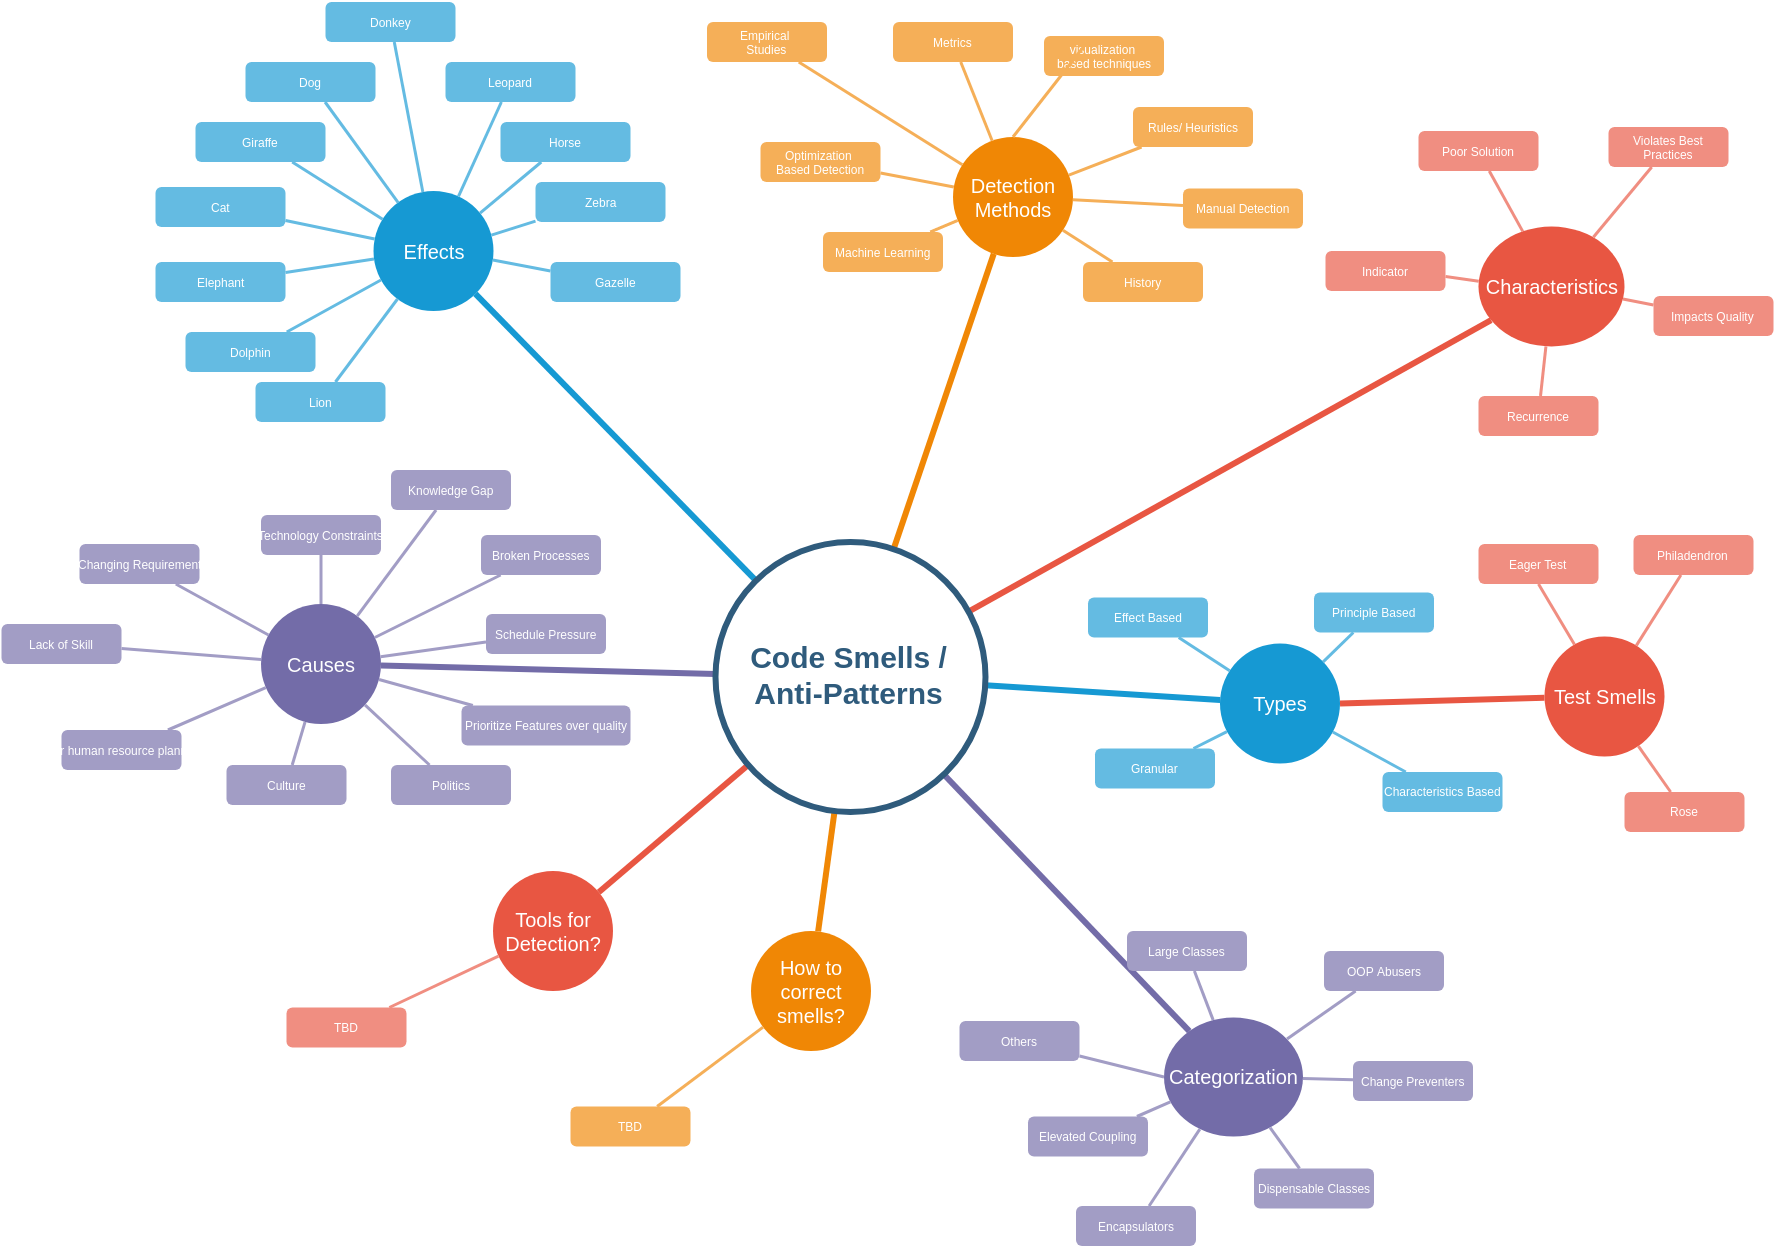
\includegraphics[width=\textwidth]{codesmells.png}}
  \caption{TopicMap}
  \label{fig:TM}
\end{figure*} 

\subsection{Notes on Survey Papers, }
For my first detailed read I chose a paper called  \textit{A survey on software smells} \cite{sharma_survey_2018}.
The following are my raw notes for this paper.

Kent Beck coined the term code smell, I should look at this paper.
Contains some ideas for topic map in abstract.
Figure 1 in paper has a pretty detailed topic map.
Interesting for comparison.
Table 4 code smells.
Interesting section on whether anti-patterns and smells synonyms, doesn't seem to be consensus. Some papers yes, some no.
Smell indicator of problem, anti pattern definitive problem.
Current detection methods cause too many false positives?
This wasn't as good as the first two papers, they did a very good job of summarizing the current research. This one talked way too much about how they did their analysis instead of the results.


For my next detailed read I chose a paper called  \textit{A systematic literature review: Refactoring for disclosing code smells in object oriented software} \cite{singh_systematic_2018}. 
The following are my raw notes for this paper.

Refers to code smells and anti-patterns interchangeably.
Related work is basically a background.
Included 238 of an initial 1053 articles.
Wow, that is a ton of papers.
The papers they drew from were on the following topics: Refactoring, anti-patterns, code smells, Object Oriented Design and refactoring, fault tolerance and OOD, SW Metrics and anti-patterns, anti-patterns in cross company projects.
Provide a lot of detail on the detection methods
Interesting to show charts based on the publisher, Conference proceedings and IEEE were top sources.


For my next detailed read I chose a paper called  \textit{Smells in software test code: A survey of knowledge in industry and academia} \cite{garousi_smells_2018}. 
The following are my raw notes for this paper.

Interesting variation on the idea of anti pattern: "test smells".
Poorly designed tests.
Really weird figures in this paper, copy paste screenshots out of spreadsheet and websites like google.
Just make a table!
They are missing the visualization, they are showing tons of tables instead of the results of the research.
Missing the analysis?


The files for this latex document are in the github repository located at \path{https://github.com/rodger79/CS6000}

Relevan papers are referenced in the bibliography below. 

\subsection{Journal4}
For my learning process so far, I've looked at how to use google scholar to optimize my time looking for the latest research.
Up until this class I would go onto the UCCS library website and use the research databases to find papers. 
It has been very helpful to set up my google scholar profile to automatically show the papers I can download through my UCCS credentails.
I have a couple of things on my to-do list.
I need to speak with Prof Boult about how to get a private github as a student, as that would be very useful, and I have a handful of questions I would like to get his opinion on. 
One thing I want to focus on is very recent relevant papers.
Fortunately google scholar allows you to researc only papers that have been written since a particular year.

\section{Journal 4}
\subsection{Who is the Main Character}
The main character is the anti-pattern. I need to find a way to clearly define the anti-pattern conceptually. 

\begin{lstlisting}[language=C,frame=single,caption=Example Anti-Pattern,label=pattern1]
#DEFINE M 2+3

int main() {
  int x=5, y;
  y= x * M;
  cout << y << endl;
  return 0;
}
\end{lstlisting}

There are some authors who define it as interchangeable as a code smell. 
I don't think that is correct. 
I think code smells are precursors to anti-patterns. 
Meaning that an anti-pattern is a known bad problem, where a code smell may lead to a problem.
An example anti-pattern is shown in listing \ref{pattern1}. Some developers will expect the output to be 25 and some will be 13 because they don't understand intuitively how the macro function works (the correct answer is 13).

On second thought, is the character the developer? 
And is what is interesting about it their human nature which leads them to confusion?
I would guess tha most developers think that a compiler is well-defined and bugs in code must be due to lack of understanding not code structure that is good at confusing human nature.
\subsection{What Character Traits Make them Interesting}
What's interesting about anti-patterns is that they have a very human aspect to them. 
They overlap the way humans think with the way code is written. 
They connect common ways of human misunderstanding to software development. 
Personally, I think most developers expect code to work as they understand it to. 
They don't spend a lot of time thinking about how code will work in ways they don't expect.
It is in the nature of most engineers to see things in mathematical/binary ways and ignore the human aspects to what they are working on.
Example boeing 737 max.
Code developers expected pilots to respond with typical emergency procedure, but when the errors occurred they pilots were overwhelmed by the amount of feedback they recieved in the cockpit (need reference).

\subsection{What do the Character Need to do or Get (Goal)}
The anti-patterns need to be understood and identified.
Once that happens developers can change their best practices.
The best practices should be created in such a way that the typical misunderstandings of the developer

\subsection{Why is That Goal Important (motive)}
Note: not many papers about code smells talk about why it is important.

\subsection{What Conflicts/Problems Block the Character}

The problem is people don't realize they are implementing anti-patterns at the time they are writing code.
The interesting things about it are how do we find them. 
How do we detect them, and what is the fix when we identify the problem.
\subsection{How do they Create Risk and Danger}
Because we know that the anti-patterns cause confusion in the developer, they create risk because they create unstable code. 
This is risk for the owner of the software and the customer of the developer who uses code
\subsection{What Does the Character Do (Struggles) to Reach Goal}
This is something I think is interesting, is how are these problems identified.
It isnt' enought to just use expert advice/knowledge. 
There must be a way to mathematically demonstrate or by experimentation that particular code patterns cause problems.

\subsection{What Sensory Details Will Make the Story Seem Real}
Real world examples of the problem


\nocite{*}
\clearpage


\bibliographystyle{IEEEtran}
\bibliography{references}


\end{document}